\documentclass{beamer}
\usepackage[space,space,hyperref]{ctex}
\usepackage{caption}
\usepackage{algorithm2e}
\usepackage{float}
\usepackage{multirow}
\usepackage{graphicx}
\usetheme{pittsburgh}
\usecolortheme{whale}
\author{Zhenjia Xu}
\title{Some other applications}
\begin{document}
	\frame{\titlepage}
	\begin{frame}[c]\frametitle{Meet in the middle}
		\begin{columns}
			\column{4cm}
			\begin{itemize}
				\item<1-> an undirected graph
				\item<1-> degree is 5
				\item<1-> find path: S to T
				\item<2-> dist(S, T) = L
				\item<3-> $O(4^L)$
				\item<4-> Meet in the middle
				\item<4-> $O(4^{L/2})$
			\end{itemize}
			\column{6cm}
			\only{\centering{{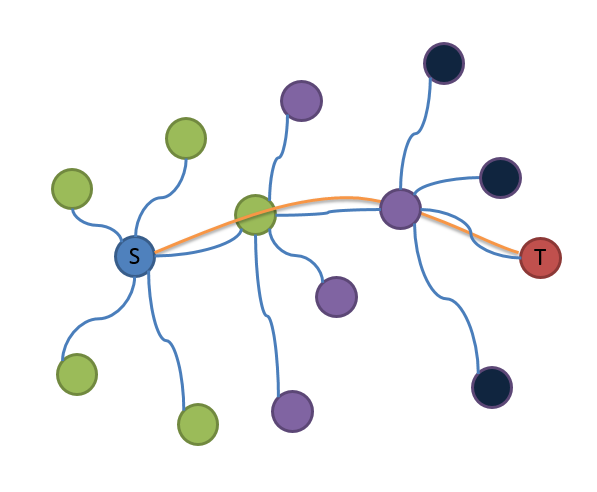
\includegraphics[width=6cm]{pic0.png}<1-2>}}}
			\only{\centering{{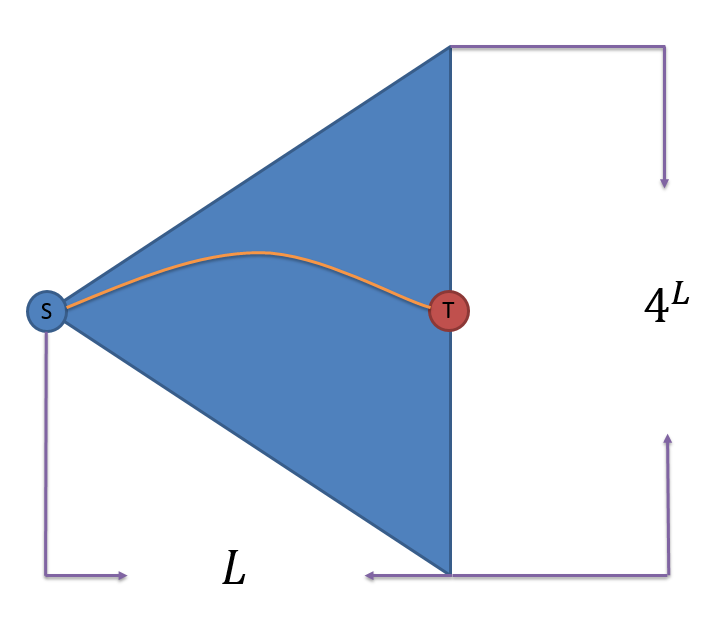
\includegraphics[width=6cm]{pic1.png}<3>}}}
			\only{\centering{{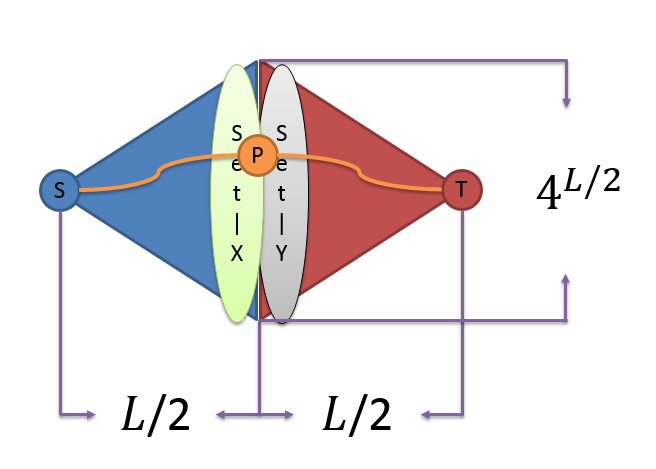
\includegraphics[width=7cm]{pic2.png}<4>}}}
		\end{columns}
	\end{frame}
	\begin{frame}[c]\frametitle{Some other applications}
		\begin{columns}
			\column{4cm}
			\beamerdefaultoverlayspecification{<+->}
			\begin{itemize}
				\item Mo's algorithm
				\item Bolcked list
				\item Dinic(capacity is 1)
				\item ......
			\end{itemize}
			\column{7cm}
			\only{\centering{{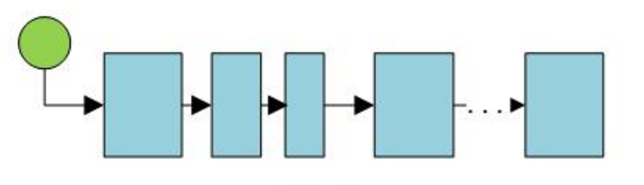
\includegraphics[width=7cm]{bl.png}<2>}}}
		\end{columns}
	\end{frame}
	
\end{document}
